\section{Aufbau}
\label{sec:Aufbau}

Der Aufbau der Apparatur ist in Abbildung \ref{fig:Aufbau} zu sehen.
Ein mit $\mathrm{Sr}^{2+}$-Ionen versetzter KBr-Kristall befindet sich in einem Gefäß, dass mit einer Vakuumpumpe verbunden und dessen Innendruck so auf $p\approx\SI{E-2}{\milli\bar}$ wurde. Der untere Teil ist mit einer Heizstromquelle verbunden und verfügt über einen Kühlfinger aus gut wärmeleitendem Material.
Die Ober- und Unterseite des Behälters besteht aus einem Plattenkondensator, der mit einem Gleichspannungsnetzgerät, einem Erdungskabel und einem Piccoamperemeter verbunden werden kann.

\begin{figure}
	\centering
	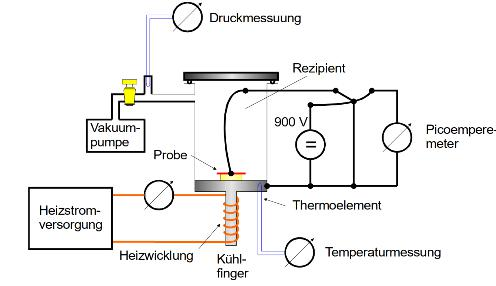
\includegraphics[width=\linewidth-70pt,height=\textheight-70pt,keepaspectratio]{content/images/Aufbau.jpg}
	\caption{Schematischer Aufbau des Versuchs \cite{V18}.}
	\label{fig:Aufbau}
\end{figure}
